\documentclass[../thesis.tex]{subfiles}

\begin{document}

\subsection{Parallel performance of HDNS with lubrication\label{sec:per}}
The second part of the discussion in this section deals with the performance of this parallel HDNS implementation that accounts for lubrication effects. To analyze the performance, a series of tests have been performed. The computational cost has been estimated for various values of the following parameters: the number of particles $N_\text{p}$, their radius $a_\text{p}$, the size of the normalized distance in which lubrication is considered $\delta$, and the number of CPU cores utilized to simulate the same system $n_\text{c}$. It should be noted that the effects of gravity are entirely neglected and in all simulations only non-settling particles are considered. Also, the simulations here are not limited to the grid resolution $64^3$, and the performance is examined at larger resolutions. The results are presented in terms of three major operations in the code: (i) the time to evolve the turbulent flow field $t_\text{FLOW}$, (ii) the time for all particle operations discussed above except for their aerodynamic interaction $t_\text{PART}$, and (iii) the time to assess their aerodynamic interaction $t_\text{AI-TOT}$ which is the sum of times for their long-range drag forces from the superposition method $t_\text{AI-HDNS}$ and their short-range lubrication interactions from analytical solutions $t_\text{AI-LUB}$. Each task includes calculations and communications. For the performance analysis here, the wall-clock times of these two operations are summed up. The colors chosen for the curves correspond with those in the algorithm presented earlier in Figure~\ref{alg}. 

The first step preceding performance tests is to generate a turbulent particle-free flow field. Beginning from a random field, the flow is evolved to a fully developed homogeneous isotropic turbulence that will be used for simulations with different settings ($N_\text{p}$, $a_\text{p}$, etc.). This stage lasts five eddy turnover times, where one eddy turnover time corresponds roughly the time scale of the largest eddies in the domain. The particles are then added to the domain at random locations and each case is run for five particle response times. This relaxation time reduces the effect of initial random distribution of particles. (This time, however, might not be enough for particles to reach a statistically stationary stage where the averages in particle statistics remain unchanged over time; see Section 3.4 in \cite{AGW07}.) Data collection is carried out over five subsequent particle response times.

The performance of this implementation is analyzed by running the tests on Okeanos supercomputer installed with the Intel Haswell Cray XC40 architecture at the Interdisciplinary Centre for Mathematical and Computational Modelling (ICM), University of Warsaw. The machine has 1084 nodes, each containing 128~GB of RAM and two 12-core Intel Xeon E5-2690 processors running at 2.6~GHz. All system nodes are connected by an ultra-scalable Cray Aries network with Dragonfly topology.



\subsubsection{Number of particles}

\begin{figure}%%%%%%%%%%%%%%%%%%%%%%%%%%%%%%%%
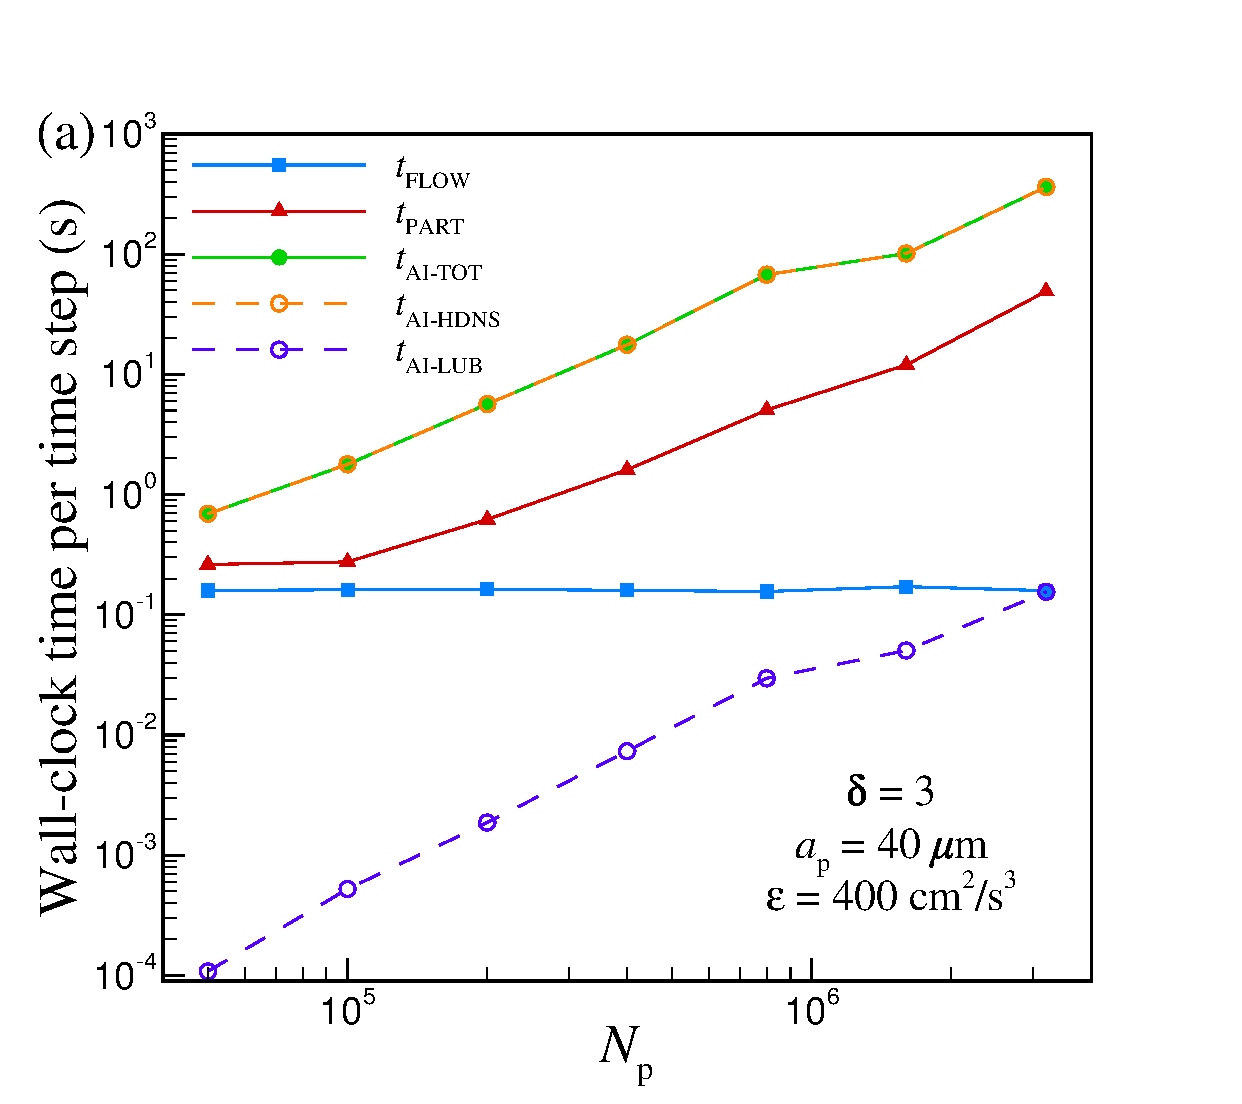
\includegraphics[trim=5mm 0mm 20mm 15mm, clip, width=0.5\textwidth]{./figs/PPAM/3a/CP022_fig3a.pdf}
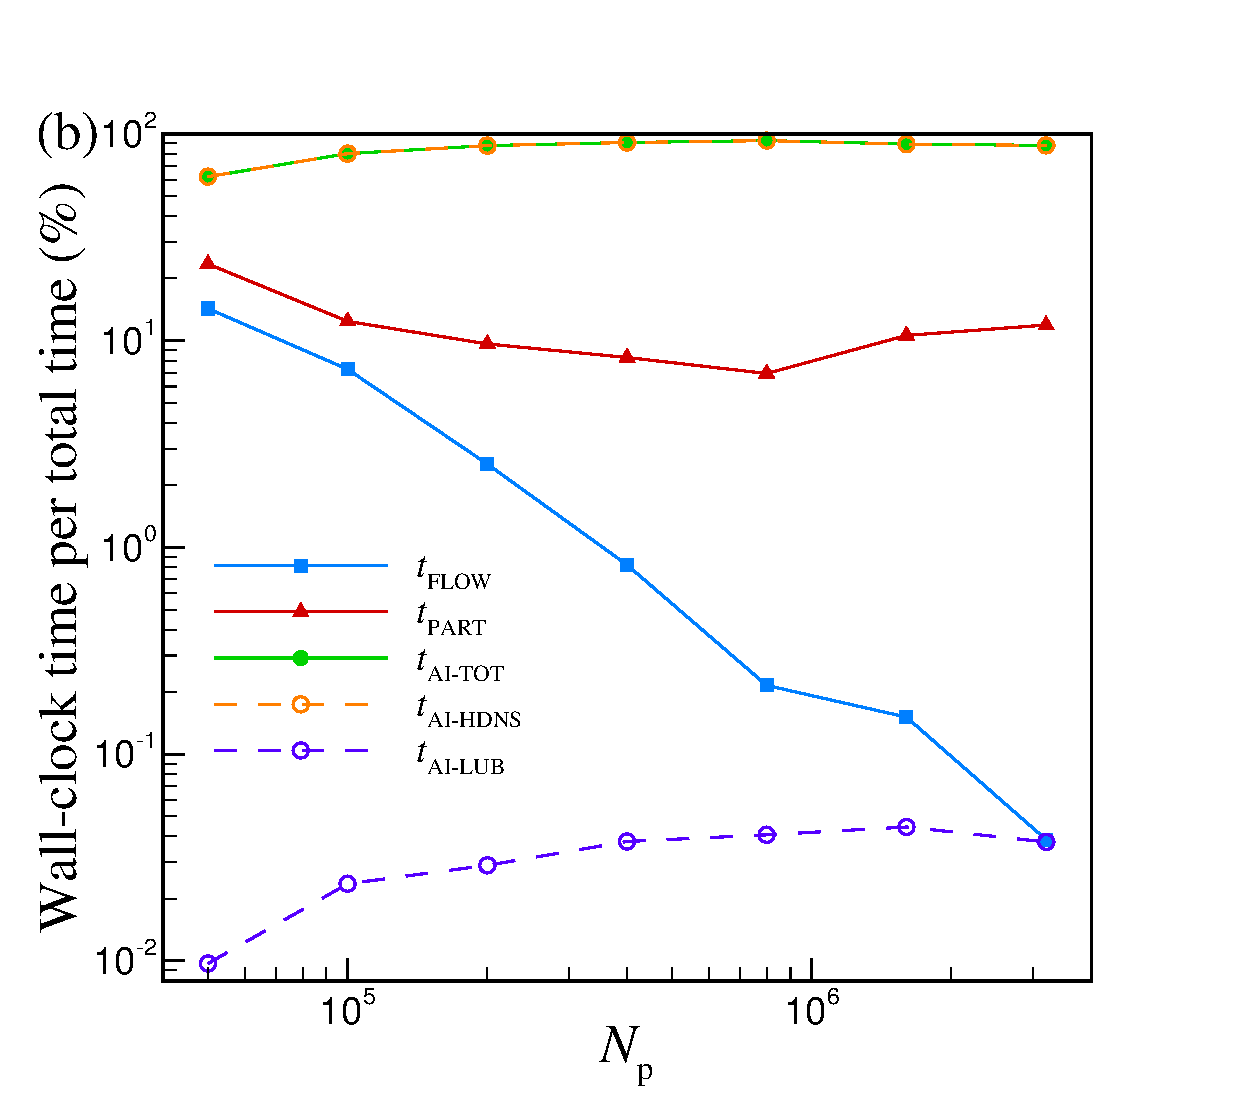
\includegraphics[trim=5mm 0mm 20mm 15mm, clip, width=0.5\textwidth]{./figs/PPAM/3b/CP022_fig3b.pdf}
\caption{Wall-clock time (a) per time step and (b) per total simulation time of different tasks as a function of the number of particles}
\label{npart}
\end{figure}%%%%%%%%%%%%%%%%%%%%%%%%%%%%%%%%%%%%%

The number of particles (droplets) in the domain is the main factor contributing to all the tasks related to particles. In Figure~\ref{npart}(a), the average wall-clock time of the selected operations per single time step is displayed as a function of the number of particles for $N_\text{p}=\{0.5$, 1, 2, 4, 8, 16, 32$\}\times10^5$. Thus, for this range of $N_\text{p}$, the average number per cell, i.e.\ $N_\text{p}/64^3$, would roughly be 0.2 to 12 particles. The droplets were of the same size $40~\mu$m for which the inertial response time of the particles $\tau_\text{p}$ is roughly equal to the Kolmogorov time scale of the flow $\tau_\text{K}$, leading to the Stokes number unity where $St = \tau_\text{p}/\tau_\text{K}$. Therefore, the particles are strongly affected by the smallest scales of the flow. It is noteworthy that having a greater number of particles in the domain enlarges the liquid water content, thus changing the phyisics of the system. Still, only the performance of the model is being investigated here. The time for all particle operations, e.g.~evaluation of lubrication forces, increases with $N_\text{p}$. For the settings considered here, the calculation of long-range AI by solving large systems of linear equations from HDNS is the most time-consuming task. Conversely, the computation of the short-range lubrication forces is several orders of magnitude faster than all the other tasks because, to maximize efficiency, the values are precomputed and interpolated as needed. For long-range AI, the size of the system of equations generated is $3N_\text{p}$, yielding a net disturbance at the location of every particle along every spatial direction. Solving such a large system requires much more computational work compared to evaluation of short-range AI forces, which basically reduces to a simple interpolation.

Integrating the equations of motion of particles, interpolating fluid velocity at particle locations, and post-processing (collision detection and computing other collision statistics including radial relative velocity and radial distribution functions) take less time, approximately one order of magnitude, than all operations related to AI. The total time for numerical operations handling particle dynamics can be compared with the time required to simulate the turbulent flow. The time needed to model the particle-free flow is the same in each considered case. As shown, computing AI forces can be one ($N_\text{p}=10^5$) to three ($N_\text{p}=3.2\times10^6$) orders of magnitude more time-consuming than evolving the turbulent flow field at $64^3$ resolution considered here. However, at larger resolutions, e.g.~$512^3$ or $1024^3$, advancing the flow field is a significantly more complex operation which can be (depending on LWC) more demanding than all particle tasks (see Figure~4 in \cite{APCRW14}).

In order to provide a relative comparison between different cases, their percentage of the total time is presented in Figure~\ref{npart}(b). There is a reduction in the shares of flow and particle wall-clock time with $N_\text{p}$ because computing AI via both HDNS and lubrication forces takes a larger fraction of the total simulation time. For instance, in simulation with \mbox{$N_\text{p}=5\times10^4$} AI takes 60\% of the total time whereas for \mbox{$N_\text{p}=3.2\times10^6$} the contribution rises to 90\%.


\subsubsection{Size of the particles}

\begin{figure}%%%%%%%%%%%%%%%%%%%%%%%%%%%%%%%%
\center
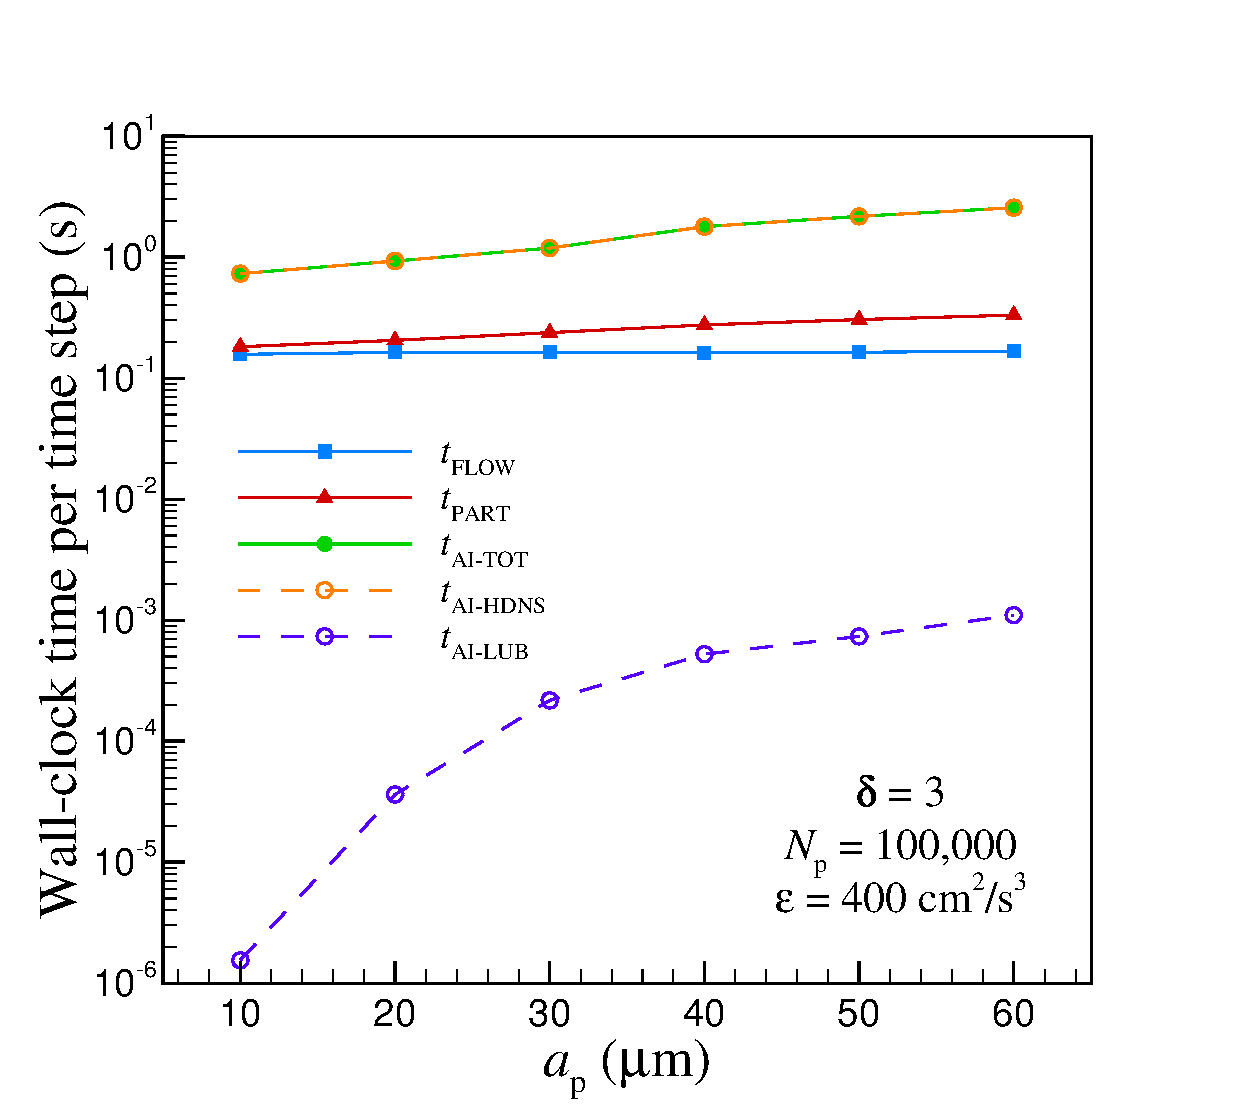
\includegraphics[trim=5mm 0mm 20mm 15mm, clip, width=0.6\textwidth]{./figs/PPAM/4b/CP022_fig4b.pdf}
\caption{Variation in the wall-clock time per time step for different operations with the size of particles}
\label{apart}
\end{figure}%%%%%%%%%%%%%%%%%%%%%%%%%%%%%%%%%%%%%

The liquid water content in the domain depends on the size and number of droplets. The number of particles grows exponentially by decreasing their radii or expanding size of the box. The effect of radii of the particles on the performance of the model is presented in Figure~\ref{apart}. A large enhancement ($y$--axis is in logarithmic scale) is seen for the total wall-clock time of the AI operation. A substantial contribution to this enhancement comes from the increase in the time needed to compute long-range interacting forces, while computing short-range lubrication forces has a minor influence on the increase in wall-clock time for AIs. Although having larger particles in the domain affects their dynamics, the increase in computation time for both AI tasks is largely due to the expansion of the volume that is scanned around every particle to account for the influence of its disturbance on the neighboring particles (see Figure~\ref{method}). That is, the larger the particle, the larger the size ($50a$) of the scanned volume for potential AI with other particles, and hence, the higher the possibility of finding such particles. Also, clustering in the distribution of particles is another factor that affects the time to compute the AI. Smaller particles are less willing to accumulate owing to their low inertia that is insufficient to deviate from the streamlines of the flow. On the other hand, larger particles with higher inertia tend to cluster, thereby increasing the number of AIs.

Similar to AI, particle tasks show a slight enhancement with particle radius. Data exchange is the main factor contributing to this increase in time. In order to conduct several particle operations -- e.g.~detection and relocation of particles that overlap, recording collision statistics, and computing aerodynamic interaction -- near the boundaries of every subdomain, data of the particles within a thin region of all neighboring subdomains have to be added to every subdomain. The size of this ``halo'' region depends on the size of the particles. Thus, larger particles need a thicker halo region which encompasses a larger number of particles, and hence requires a greater number of calculations and communications.


\subsubsection{Size of the short-range region}

\begin{figure}%%%%%%%%%%%%%%%%%%%%%%%%%%%%%%%%
\centering
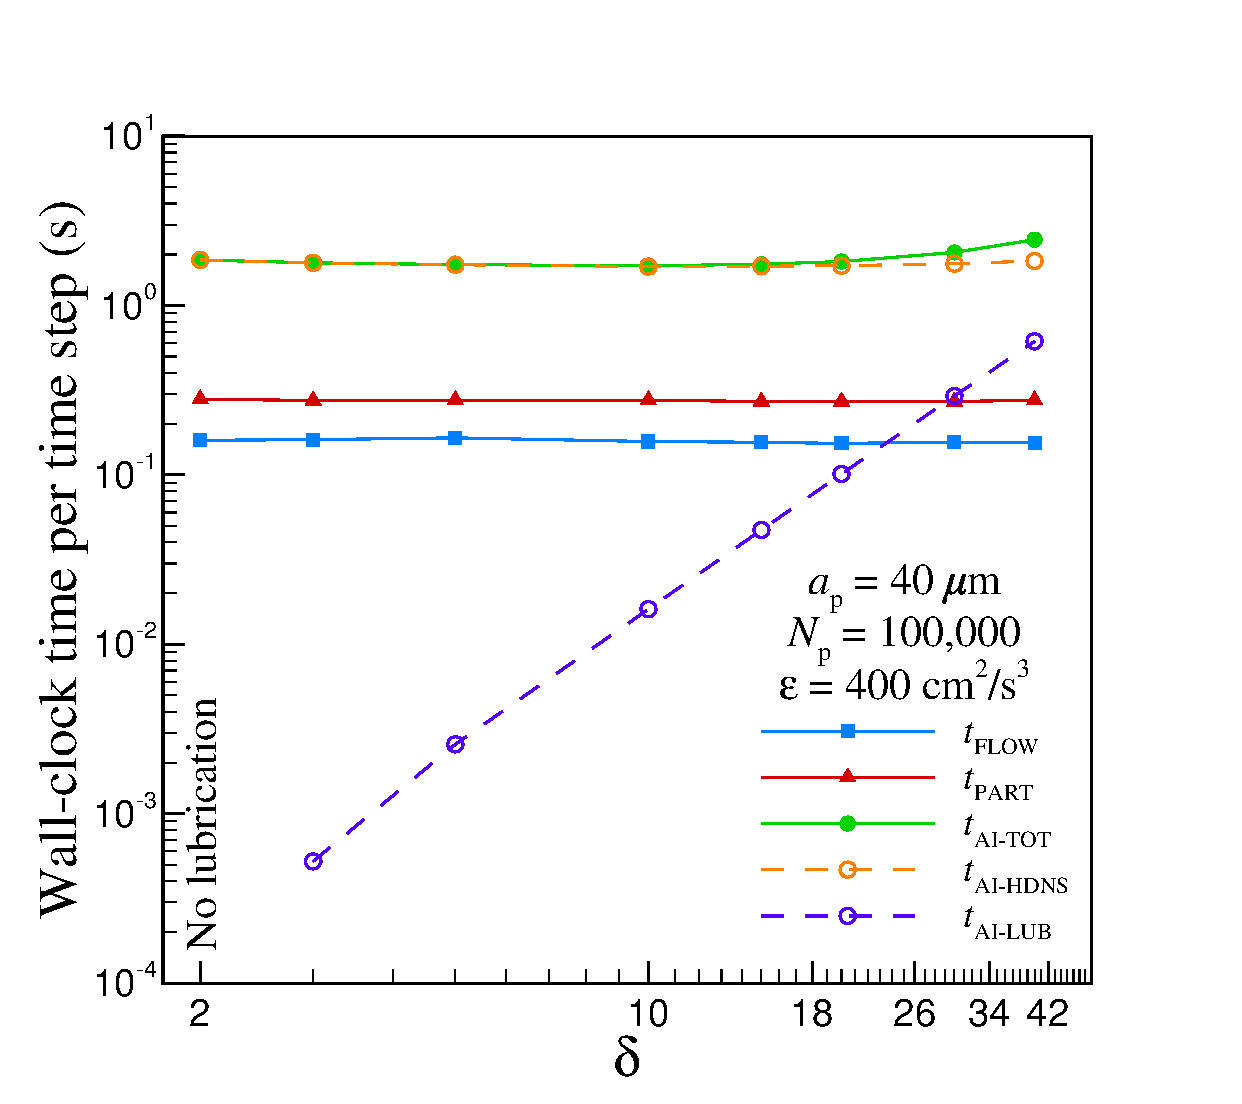
\includegraphics[trim=5mm 0mm 20mm 15mm, clip, width=0.6\textwidth]{./figs/PPAM/5/CP022_fig5.pdf}
\caption{Variation in wall-clock time of different operations per time step with the size of lubrication region}
\label{delta}
\end{figure}%%%%%%%%%%%%%%%%%%%%%%%%%%%%%%%%%%%%%

So far, the results were presented for a fixed size of the region in which lubrication forces are considered: $\delta=3$. There are two reasons for this particular choice. Firstly, the accuracy in the superposition method (HDNS) begins to decline for pairs separated at normalized distances $\delta\leq3$ (see Figure~\ref{Fig1}). For such pairs short-range lubrication forces can be obtained from the analytical solutions to the Stokes flow around \textit{two} spherical particles \citep{JO84}. Secondly, since two-sphere analytical solutions are limited to pair-wise interactions, increasing the size of lubrication region, $\delta$, results in losing the effect of many-body interaction among particles, which is taken into account by superposing perturbation induced by all neighboring particles \citep{WAG05,AGW07}. Therefore, $\delta=3$ is a~choice in between that considers the effects of both lubrication forces and many-body interaction.

Figure~\ref{delta} shows the wall-clock time required by each operation as a function of the size of lubrication region. When $\delta=2$, there is no lubrication region and AI is entirely handled by HDNS (i.e.~$t_\text{AI-LUB}=0$). As the size of lubrication region changes from one particle radius ($\delta=3$) to forty particle radii ($\delta=42$), the time to calculate lubrication forces increases by three orders of magnitude. As a~result, the total AI time (i.e.~$t_\text{AI-TOT}=0$) grows, too. The rest of the tasks do not depend on the size of lubrication region.


\subsubsection{Number of CPU cores}

\begin{figure}%%%%%%%%%%%%%%%%%%%%%%%%%%%%%%%%%%%
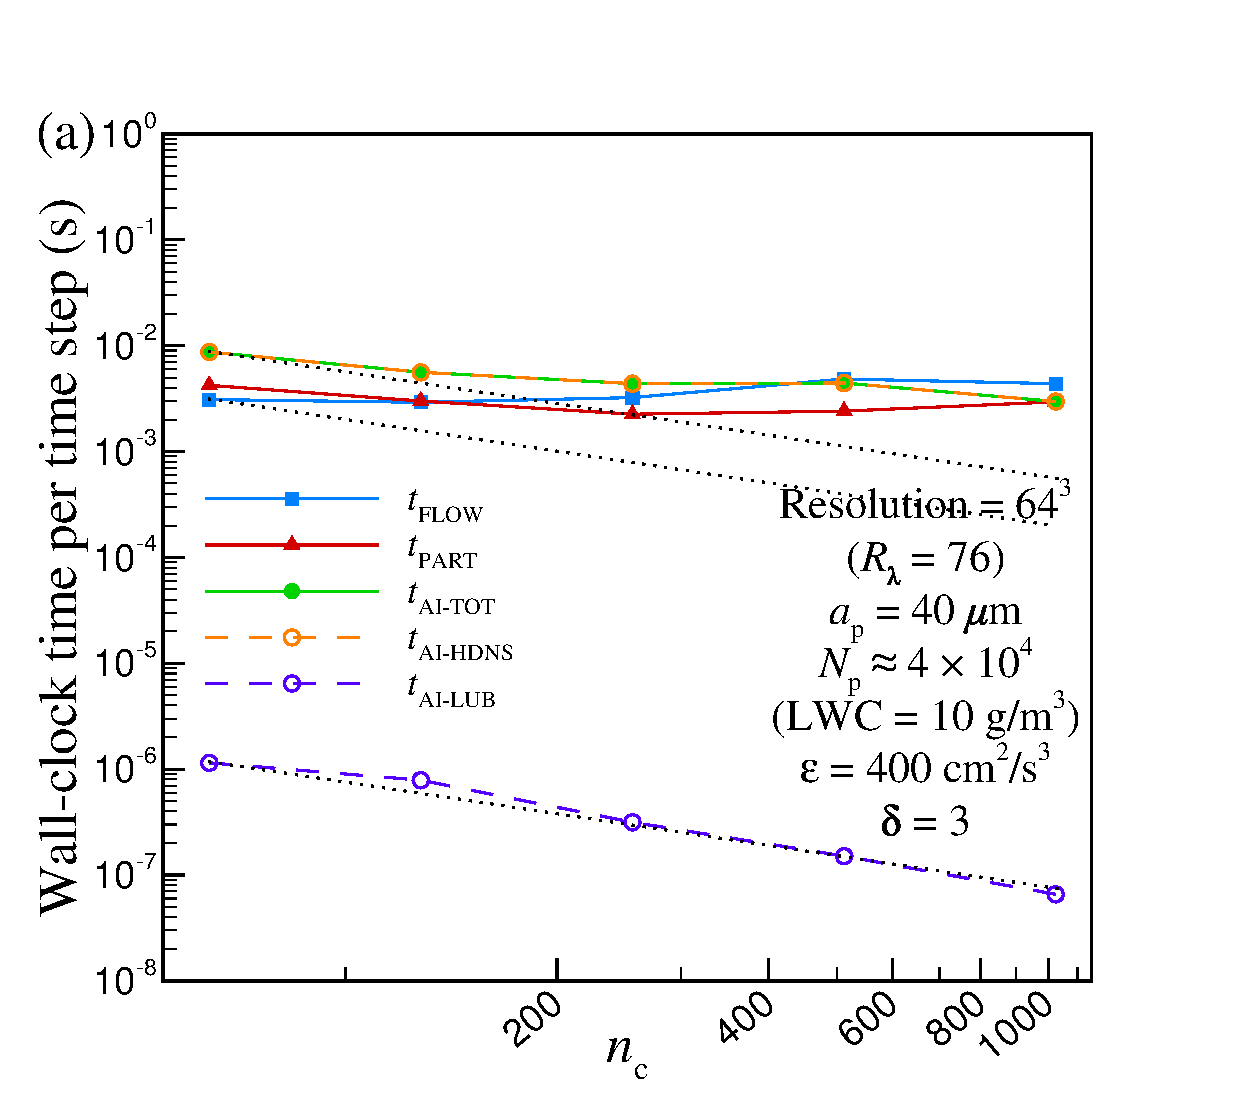
\includegraphics[trim=5mm 0mm 20mm 15mm, clip, width=0.5\textwidth]{./figs/PPAM/6a/CP022_fig6a.pdf}
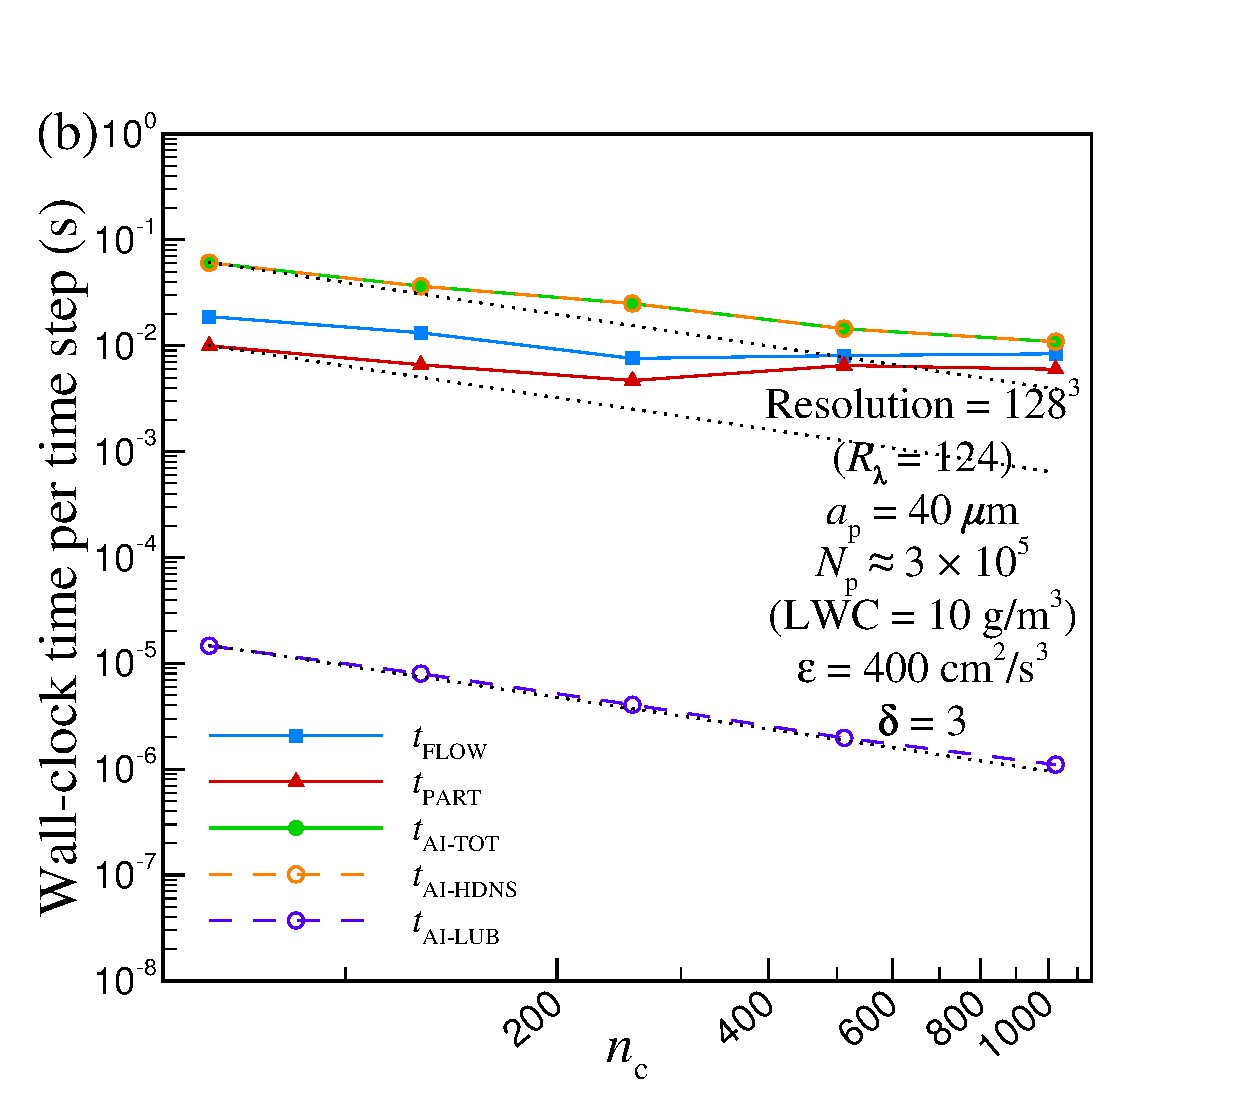
\includegraphics[trim=5mm 0mm 20mm 15mm, clip, width=0.5\textwidth]{./figs/PPAM/6b/CP022_fig6b.pdf}
\centerline{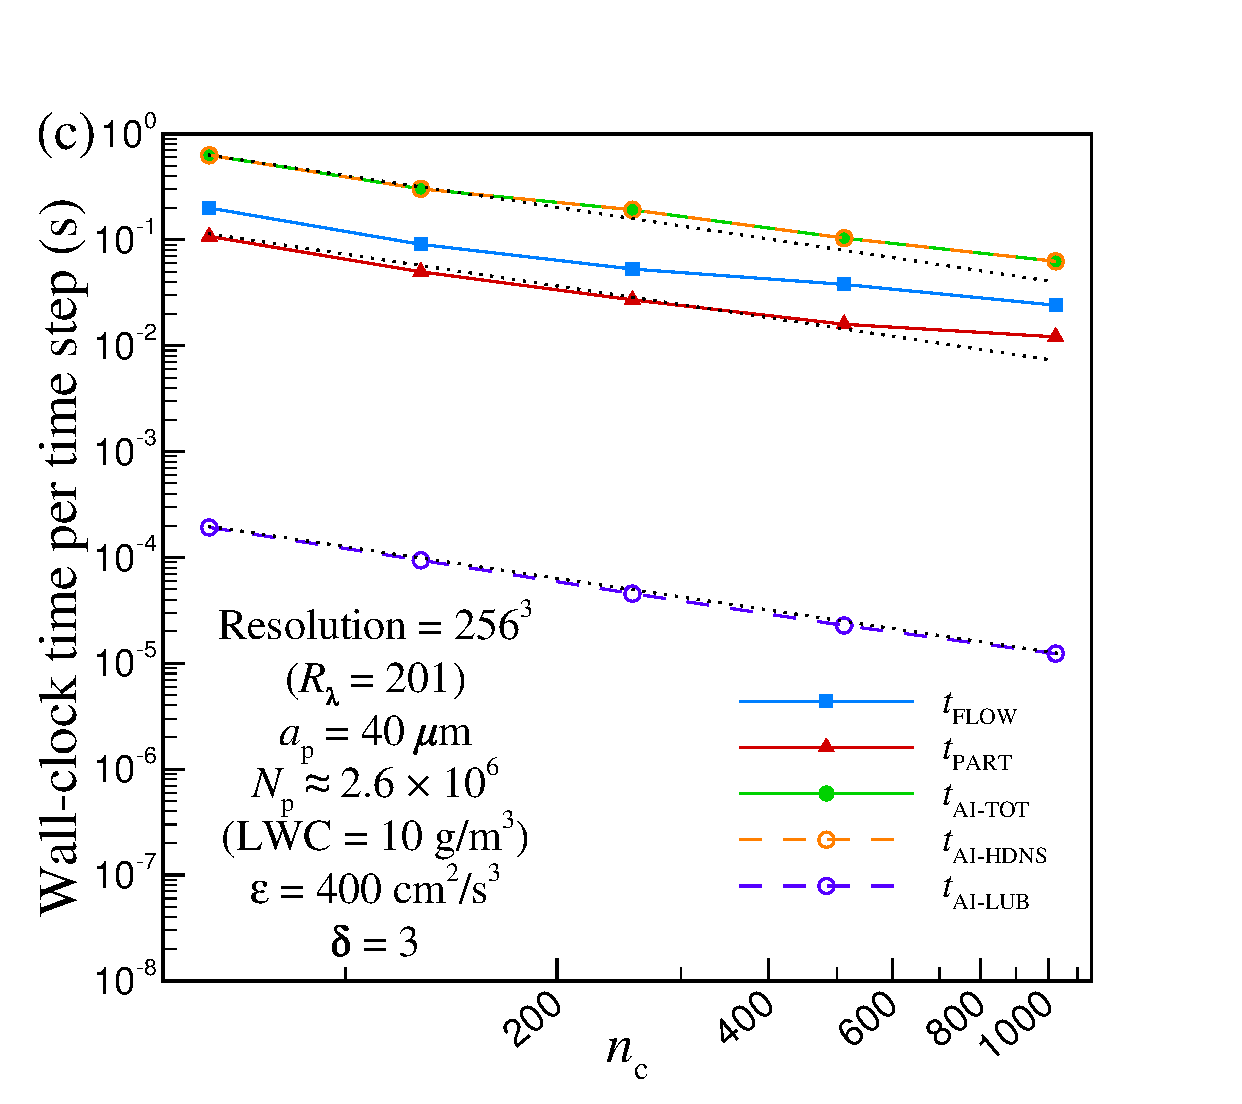
\includegraphics[trim=5mm 0mm 20mm 15mm, clip, width=0.5\textwidth]{./figs/PPAM/6c/CP022_fig6c.pdf}}
\caption{Wall-clock time per time step of different operations as a function of the number of CPU cores for three systems with the same LWC 10 g/m$^3$ and turbulent flows at resolutions: (a) $64^3$, (b) $128^3$, and (c) $256^3$ (dotted lines: \mbox{slope $=-1$)}}
\label{nproc}
\end{figure}%%%%%%%%%%%%%%%%%%%%%%%%%%%%%%%%%%%%%

Several tests have been performed to check how each task scales with the number of computational cores utilized: $n_\text{c}=2^n$ for $n=6,\dots,10$. The results are demonstrated in Figure~\ref{nproc} for three systems simulated on grids of sizes $64^3$, $128^3$, and $256^3$ with the same liquid water content 10 g/m$^3$. The range of \mbox{$y$--axis} is identical on all three panels to facilitate comparisons. Panels (a)--(c) illustrate the increase in execution time for all tasks as the domain is enlarged. In general, computing long-range aerodynamic interactions is the most time-consuming operation. This is caused by the necessity to track a large number of particles owing to the high LWC (assumed for the systems simulated here). A~large fraction of this time is due to HDNS, whereas interpolation of lubrication forces takes several orders of magnitude less time. The time to advance the flow is shorter than the time to evaluate AIs, but longer than that for particle operations (velocity interpolation, recording collision statistics, etc.). Another finding is the improvement in scalability at higher resolutions. At $64^3$, the three major tasks -- i.e.~AIs, flow, and particles -- do not show a better performance with the number of CPU cores employed. Wall-clock times of the flow and particle operations even begin to increase when more than 256 cores are used. Scalability slightly improves at the higher resolution $128^3$ displaying a logarithmic decrease in computation time, again, until $n_\text{c}=256$. However, using a larger number of cores does not lead to a lower wall-clock time for advancing the flow and particle operations. The best performance is observed at the resolution $256^3$ showing a~logarithmically decreasing time with the number of processors used.

\subsubsection{Summary}
The analysis here was aimed at examining the parallel performance of a novel implementation for tracking inertial particles in turbulent flows. This code serves for modeling cloud processes and investigating the role of turbulence on the droplet collision rate. The computational performance was assessed based on a number of testing simulations by measuring the time required to conduct individual operations. The focus was on computation time for aerodynamic interaction and lubrication forces, and the results were directly compared with the time required for the other tasks related to droplet tracking and computing collision statistics as well as the time to advance the turbulent flow field. The factors examined here were the number and size of the particles in the domain, the size of the region in which lubrication effects are considered, and the number of processors to simulate three different systems. The first three factors increased computation time. It has been observed that the scalability of the code improves with increasing resolution of the computational grid. This is an encouraging perspective to run simulations on even larger computational meshes, or equivalently larger Reynolds numbers. Therefore, the approach makes it possible to conduct simulations in conditions more similar to those in realistic clouds. This leads to the development of more realistic parameterizations for weather forecasting models.

%\bibliographystyle{bibstyle}
%\bibliography{references}
\newpage
\end{document}
